% Kopfzeile beim Kapitelanfang:
\fancypagestyle{plain}{
%Kopfzeile links bzw. innen
\fancyhead[L]{\Large Vorlesung 24 (16.01.2013)}
%Kopfzeile rechts bzw. außen
\fancyhead[R]{}}
%Kopfzeile links bzw. innen
\fancyhead[L]{\Large Vorlesung 24 (16.01.2014)}
%Kopfzeile rechts bzw. außen
\fancyhead[R]{}
% **************************************************
\section{Definition: Supremumsnorm}\label{13.3}
Sei $f: D \to \R$ eine Funktion.\\
$||f||_D := \sup_{x \in D} |f(x)|$ \underline{Supremumsnorm} von $f$ auf $D$\nl
Damit:
\en{
\item $f$ beschränkt $\Lra ||f||_D < \infty$
\item $f_n \to f$ gleichmäßig auf $D \Lra \lim_{n \to \infty} ||f_n-f||_D = 0$
}

\subsection*{Beispiele}
\en{
\item $f_n(x) = \frac{\sin(n x)}{n}$ auf $D=\R$
$||f_n||_\R = \frac{1}{n} \Ra f_n \to 0$ gleichmäßig auf $\R$
\item $f_n(x) = x^n$ auf $[0,1]$\\
$f(x) = \left\{\begin{array}{l l} 0 & x \in [0,1) \\ 1 & x=1 \end{array}\right.$\\
$f_n \to f$ punktweise, aber \underline{nicht} gleichmäßig auf $[0,1]$\\
Denn: $0 < \eps < 1 \Ra \forall n \in \N \exists x_n \in [0,1): f_n(x_n) > \eps$, aber $f(x_n) = 0$\\
$||f_n-f||_{[0,1]} = 1$
}

\section*{Eigenschaften von $||\ldots||$}
\en{
\item $||f||_D \ge 0$ und $||f||_D = 0 \Lra f=0$ (Definitheit)
\item $\lambda \in \R \Ra ||\lambda f||_D = |\lambda| \cdot ||f||_D$ (Homogenität)
\item $||f+g||_D \le ||f||_D + ||g||_D$ (Dreiecksungleichung),\\
denn: $|f(x)+g(x)| \le |f(x)|+|g(x)| \Ra \sup_{x \in D} |(f+g)(x)| \le \sup_{x \in D} |f(x)| + \sup |g(x)|$
}

\section{Satz}\label{13.4}
Sei $f_n: D \to \R$ eine Folge \underline{stetiger} Funktionen, die gleichmäßig gegen $f: D \to \R$ konvergiert $\Ra$ auch $f$ ist stetig auf $D$.

\subsection*{Beweis}
Sei $x_0 \in D$. Zu zeigen: $\forall \eps > 0 \exists \delta > 0: |f(x)-f(x_0)| < \eps \forall x \in D$ mit $|x-x_0| < \delta$\\
Dazu: $f_n \to f$ gleichmäßig $\Ra \exists N \in \N: ||f_N-f||_D < \frac{\eps}{3}$ (*)\\
$f_N$ stetig in $x_0 \Ra \exists \delta > 0: |f_N(x)-f_N(x_0)| < \frac{\eps}{3} \wedge \forall x \in D: |x-x_0| < \delta$\nl
Für diese $x$ folgt: $|f(x)-f(x_0)| \le$ Trick!\\
$\underbrace{|f(x)-f_N(x)|}_{< \frac{\eps}{3} \text{aus (*)}} + \underbrace{|f_N(x)-f_N(x_0)|}_{< \frac{\eps}{3}} + \underbrace{|f_N(x_0)-f(x_0)|}_{< \frac{\eps}{3}} < \eps$ \qed

\newpage

\section*{Gleichmäßig konvergente Funktionsreihen}
Gegeben: $f_n: D \to \R$ ($n \in \N$)
Def.: $\sum_{n=1}^\infty f_n: D \to \R: \left(\sum_{n=1}^\infty f_n\right)(x) := \sum_{n=1}^\infty f_n(x)$ sofern konv. $\forall x \in D$

\subsection*{Beispiel}
$f_n(x) = \frac{x_n}{n!}$ auf $\R \Ra \left(\sum_{n=0}^\infty f_n\right)(x) = \sum_{n=0}^\infty \frac{x^n}{n!} = e^x$

\section{Definition}\label{13.5}
$\sum_{n=1}^\infty f_n$ heißt gleichmäßig konvergent auf $D :\Lra$\\
die Folge der Partialsummen $g_n(x) = \sum_{k=1}^n f_k(x), n \in \N$ konvergiert gleichmäßig auf $D$.

\subsection*{Satz \ref{13.4} zeigt}
Ist $\sum_{n=1}^\infty f_n$ gleichmäßig konvergent auf $D$ und alle $f_n$ stetig auf $D$\\
$\Ra f(x)=\sum_{n=1}^\infty f_n(x)$ ist stetig auf $D$.

\section{Kriterium von Weierstraß}\label{13.6}
Seien $f_n: D \to \R$ mit $\sum_{n=1}^\infty ||f_n||_D < \infty \Ra$\\
$\Ra \sum_{n=1}^\infty f_n$ konvergiert absolut und gleichmäßig auf $D$\\
("`konvergiert absolut auf $D$"' heißt: $\sum_{n=1}^\infty |f_n(x)| < \infty \forall x \in D$)

\subsection*{Beispiel}
$\sum_{n=1}^\infty \underbrace{\frac{\cos(nx)}{n^2}}_{=f_n(x)} =: f(x)$ konvergiert absolut und gleichmäßig auf $\R$.\\
Denn: $\sum_{n=1}^\infty ||f_n||_\R = \sum_{n=1}^\infty \frac{1}{n^2} < \infty$. Weierstraß $\Ra$ Behauptung.\\
Alle $f_n$ stetig auf $\R \Ra f$ stetig auf $\R$.

\subsection*{Beweis}
Absolute Konvergenz mit Majorantenkriterium: $\sum_{n=1}^\infty |f_n(x)| \le \underbrace{\sum_{n=1}^\infty ||f_n||_D}_{\text{konv. Majorante}} < \infty$\\
Sei $x \in D \Ra |f(x) - \sum_{k=1}^n f_k(x)| = |\sum_{k=n+1}^\infty f_k(x)| \le \sum_{k=n+1}^\infty |f_k(x)| \le \sum_{k=n+1}^\infty ||f_k||_D = c_n$ gleichmäßig in $x$!\\
$\Ra ||f-\sum_{k=1}^n f_k||_D \le c_n \underset{n \to \infty}{\to} 0$ \qed

\section{Gleichmäßige Konvergenz komplexer Funktionen}\label{13.7}
Alle bisherigen Definitionen und Sätze zur gleichmäßigen Konvergenz (insbes. Weierstraßkriterium) übertragen sich wörtlich auf Folgen und Reihen komplexer Funktionen $f_n: D \to \C, D \subseteq \C$.

\section*{Potenzreihen}
Exponentialreihe: $\sum_{n=0}^\infty \underbrace{\frac{z^n}{n!}}_{f_n(z), z \in \C} = e^z$

\section{Definition: Potenzreihen}\label{13.8}
Eine \underline{Potenzreihe} ist eine Reihe der Form
$$\sum_{n=0}^\infty c_n(z-a)^n, z \in \C$$
mit Koeffizienten $c_n \in \C$\\
und Entwicklungspunkt $a \in \C$\nl
Substitution: $z-a =: z' \Ra$ Reduktion auf Fall $a=0$\\
Für welche $z \in \C$ konvergiert $\sum_{n=0}^\infty c_n z^n$?

%\newpage

\section{Lemma}\label{13.9}
Sei $\sum_{n=0}^\infty a_n z^n$ konvergent für $z=z_0 \in \C, z_0 \neq 0$\\
$\Ra \sum a_n z^n$ konvergiert absolut und gleichmäßig auf jeder Kreisscheibe $\overline{K_r(0)} := \{z \in \C : |z| \le r\}$ (mit Rand) mit $r < |z_0|$\nl
\begin{tikzpicture}
\draw[thick,color=red] (0,0)--(0.70710678,0.70710678);
\draw[thick,color=red] (0.35355339,0.35355339) node[right] {$r$};
\draw[color=red,pattern=custom north west lines,hatchcolor=red] (0,0) circle (1);
\draw[color=blue] (0,0) circle (1.5);
\draw[thick,color=blue] (0.70710678,0.70710678)--(1.06066017,1.06066017) node[right] {$z_0$};
\draw[thick] (-0.35355339,0.35355339) node {$\bullet$} node[left] {$z$};
\draw (1.3,-1.3) node[right] {$r < |z_0|$};
\end{tikzpicture}

\subsection*{Beweis}
$\sum c_n z_0^n$ konvergiert $\Ra \exists M > 0: |c_n z_0^n| \le M \forall n \in \N$\\
$f_n(z) = c_n z^n, r < |z_0|$\\
$\Ra ||f_n||_{\overline{K_r(0)}} = \sup_{|z| \le r} |c_n z^n| = |c_n| \cdot r^n \underset{\text{Trick}}{=} |c_n z_0^n| \cdot \frac{r^n}{|z_0^n|} \le M \cdot \left(\frac{r}{|z_0|}\right)^n = M q^n$ mit $q=\frac{r}{|z_0|} < 1$\\
$\sum_{n=0}^\infty (M q^n) < \infty$ (geom. Reihe) $\underset{\text{Weierstr.}}{\Ra}$ Behauptung. \qed

\section{Definition: Konvergenzradius}\label{13.10}
Konvergenzradius der Potenzreihe $\sum_{n=0}^\infty c_n z^n$:\\
$R := \sup \{r>0: \sum_{n=0}^\infty c_n r^n \text{ konv.}\}$ ($R := \infty$, falls konv. $\forall r \le 0$)

\section{Satz}\label{13.11}
\begin{tikzpicture}
\draw[color=red,pattern=custom north west lines,hatchcolor=red] (0,0) circle (1);
\draw[color=blue] (0,0) circle (1.5);
\draw[color=red] (0,0) node {$\bullet$} node[below] {$0$};
\draw[color=blue] (1.5,0) node {$\bullet$} node[right] {$R$};
\draw[color=blue] (-1.06066017,1.06066017)--(-1.41421356,1.41421356) node[left] {ohne Rand konv.};
\draw[color=red] (-0.70710678,-0.70710678)--(-1.41421356,-1.41421356) node[left] {gleichmäßig konv.};
\end{tikzpicture}
\en{
\item $|z| < \R \Ra \sum_{n=0}^\infty c_n z^n$ konvergiert absolut, und die Konvergenz ist gleichmäßig auf jeder Kreisscheibe $\overline{K_r(0)}$ mit $r < R$
\item $f(z) = \sum_{n=0}^\infty c_n z^n$ ist stetig in $K_R(0) = \{z \in \C: |z| < R\}$
\item $|z| > R \Ra \sum c_n z^n$ divergiert
}

\subsection*{Beweis}
\en{
\item Sei $r > R$. Wähle $r_0$ mit $r < r_0 < R \underset{\text{Def. von R}}{\Ra} \sum c_n r_0^n$ konv.\\
Lemma \ref{13.9} $\Ra$ absolut und gleichmäßige Konvergenz in $\overline{K_r(0)}$.\nl
\begin{tikzpicture}
\draw (-1,0)--(2,0);
\draw[color=blue,pattern=custom north west lines,hatchcolor=blue] (0,0) circle (0.5);
\draw (0,0) node {$\bullet$} node[below] {$0$};
\draw[color=red] (0.5,0) node {$\bullet$} node[below] {$r$};
\draw[color=red] (1,0) node {$\bullet$} node[below] {$r_0$};
\draw[color=red] (1.5,0) node {$\bullet$} node[below] {$R$};
\end{tikzpicture}
\item $f_n(z) = c_n z^n$ auf $\C \underset{\text{(1)}}{\Ra} f$ stetig auf jeden $\overline{K_r(0)}$ mit $r < R$
\item Sei $|z| > R$. Angenommen, $\sum c_n z^n$ konvergiert. $\underset{\text{\ref{13.9}}}{\Ra} \sum c_n r^n$ konv. $\forall r$ mit $R < r < |z|$ \wspruch zu Def. von $R$\nl
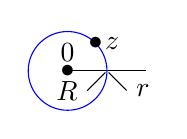
\begin{tikzpicture}
\draw (0,0)--(1,0);
\draw[color=blue] (0,0) circle (0.5);
\draw (0,0) node {$\bullet$} node[above] {$0$};
\draw (0.35355339,0.35355339) node {$\bullet$} node[right] {$z$};
\draw (0.48,-0.02)--(0.25,-0.25) node[left] {$R$};
\draw (0.52,-0.02)--(0.75,-0.25) node[right] {$r$};
\end{tikzpicture} \qed
}

\section{Berechnung des Konvergenzradius'}\label{13.12}
Gegeben: $\sum_{n=0}^\infty c_n z^n$
\en{
\item Falls $q = \lim_{n \to \infty} \left|\frac{c_{n+1}}{c_n}\right| \in [0,\infty]$ existiert\\
$\Ra R = \frac{1}{q}$ (dabei: $\frac{1}{0} := \infty, \frac{1}{\infty} = 0$)
\item Falls $q = \lim_{n \to \infty} \sqrt[n]{|c_n|} \in [0,\infty]$ existiert\\
$\Ra R = \frac{1}{q}$
}

\subsection*{Beweis}
\en{
\item $\left|\frac{c_{n+1} z^{n+1}}{c_n z^n}\right| \underset{n \to \infty}{\to} q \cdot |z| \left\{\begin{array}{l l} <1 & \text{falls } |z| < \frac{1}{q} \\ >1 & \text{falls } |z| > \frac{1}{q}\end{array} \right. \Ra R = \frac{1}{q}$
\item Analog mit Wurzelkriterium (T2, Blatt 6) $\sqrt[n]{|c_n z^n|} \to q \cdot |z|$
} \qed

\section{Beispiel}\label{13.13}
\enk{
\item $e^z = \sum_{n=0}^\infty \frac{z^n}{n!}$\\
Da konv. $\forall z \in \C$, muss $R = \infty$ sein.\\
Berechne mit (1): $c_n = \frac{1}{n!}, \left|\frac{c_{n+1}}{c_n}\right| = \frac{n!}{(n+1)!} = \frac{1}{n+1} \underset{n \to \infty}{\to} 0 \Ra q=0, R=\infty$
}